\documentclass[10pt]{article}

\usepackage[margin=0.72in]{geometry}
\usepackage[T1]{fontenc}
\usepackage{lmodern}
\usepackage{titlesec}
\usepackage{enumitem}
\usepackage{xcolor}
\usepackage{graphicx}
\usepackage{booktabs}
\usepackage{tabularx}
\usepackage{amsmath}
\usepackage{amssymb}
\usepackage{parskip}
\usepackage[most]{tcolorbox}
\usepackage[labelfont=bf,font=small]{caption}
\usepackage{float}
\usepackage{hyperref}

\definecolor{ink}{HTML}{1F2933}
\definecolor{acc}{HTML}{0F9D8A}
\definecolor{soft}{HTML}{E6FCF5}

\titlespacing*{\section}{0pt}{1em}{3pt}
\titlespacing*{\subsection}{0pt}{0.8em}{2pt}
\titleformat{\section}{\normalfont\large\bfseries}{\thesection}{0.6em}{}
\titleformat{\subsection}{\normalfont\bfseries}{\thesubsection}{0.6em}{}
\setlist{itemsep=1pt, topsep=2pt, parsep=0pt}

% Code blocks in a dark box, matching the team's usual report convention.
\newtcblisting{shellcode}{
    listing only, breakable,
    colback=black!95!white, colframe=black!80!white, boxrule=1pt,
    listing options={basicstyle=\ttfamily\footnotesize\color{white}, columns=fullflexible,
                     breaklines=true, keepspaces=true, showstringspaces=false}
}
\newtcolorbox{keybox}{colback=soft, colframe=acc, boxrule=0.8pt, arc=3pt, left=6pt, right=6pt, top=4pt, bottom=4pt}

\hypersetup{colorlinks=true, linkcolor=black, urlcolor=black, citecolor=black}
\setlength{\parindent}{0pt}
\setlength{\parskip}{3pt}
\graphicspath{{../figures/}{diagrams/}}

\begin{document}

\begin{center}
{\Large \textbf{Technical Document: Frame-Level Ball Possession}}\\[3pt]
{\large More than a Hack 2027, Phase 1, FC Barcelona vs Athletic Club}\\[5pt]
Team \textit{False Five}\\[2pt]
Farrel Athalla Putra, Izhar Alif Akbar, Raka Daffa Iftikhaar, Kefas Kurnia Jonathan, M. Fithra Rizki\\[2pt]
\small Code: \url{https://github.com/farrelathalla/False-Five---More-Than-A-Hack-2027}
\end{center}

\begin{keybox}
\textbf{In Short}
\begin{itemize}[leftmargin=1.2em]
\item Possession is learned from \textbf{74 fully labelled professional matches} (DFL Bundesliga, Metrica sample games, PFF World Cup 2022), each degraded with \textbf{BAR-ATH's own ball gaps, player dropouts and position bias}, and aligned to one notion of \emph{controlled} possession.
\item Two BiGRUs and two dilated TCNs read up to 100 s of team-level context around every frame. A greedy ensemble is selected on held-out spellF1, and a \textbf{duration-constrained three-state Viterbi} turns probabilities into possessions.
\item Broadcast replays and the length of ball-tracking gaps enter the dead-ball state as explicit evidence terms, each one cross-checked by the other.
\item Held-out spellF1 \textbf{0.771} on 52 halves from three leagues (macroF1 0.923). Public window: spellF1 \textbf{0.688} vs 0.424 for the best baseline, macroF1 \textbf{0.927}. The CSV is regenerated \textbf{byte for byte} in seconds.
\end{itemize}
\end{keybox}

\section*{Problem Overview}
For each of the 199{,}319 frames of the tactical video, the task is to output \texttt{H} (Barcelona has the ball), \texttt{A} (Athletic has the ball), \texttt{D} (the ball is dead) or \texttt{X} (abstain). Ranking uses spellF1. A possession is a maximal run of \texttt{H} or of \texttt{A}, predicted and true possessions are matched one-to-one by temporal IoU, and F1 is averaged over five thresholds,
\begin{equation}
\text{spellF1} = \frac{1}{5}\sum_{\theta \in \{0.3,0.4,0.5,0.6,0.7\}} \frac{2\,TP_\theta}{2\,TP_\theta + FP_\theta + FN_\theta},
\end{equation}
with macroF1 over \texttt{H}, \texttt{A}, \texttt{D} as the tie-break. Graded frames are 11{,}185 to 90{,}651 and 110{,}808 to 190{,}197.

\section*{The Core Challenge}
The metric rewards \emph{segmentation}, not frame accuracy. A one-second false switch invents a possession and can split a true one below the IoU threshold, so every flicker is paid twice. A dead ball splits a possession in two, which makes stoppage detection as important as the team call. A systematic one-second boundary offset costs about 0.35 spellF1 on a typical possession.

The data makes this harder. The tracking is automatic and uncorrected, player slots are tracklets rather than identities, and the ball is missing on 41\% of graded frames, mostly in long blocks with a median of 10.7 s (Figure~\ref{fig:ball}). The public window, by contrast, has the ball on 88\% of frames. It is far easier than the rest of the match and holds only 17 possessions, so one possession moves its spellF1 by about 0.06. How can a model learn possession without labelled tracking of this match, and how can it be validated without trusting five minutes?

\begin{figure}[H]
\centering
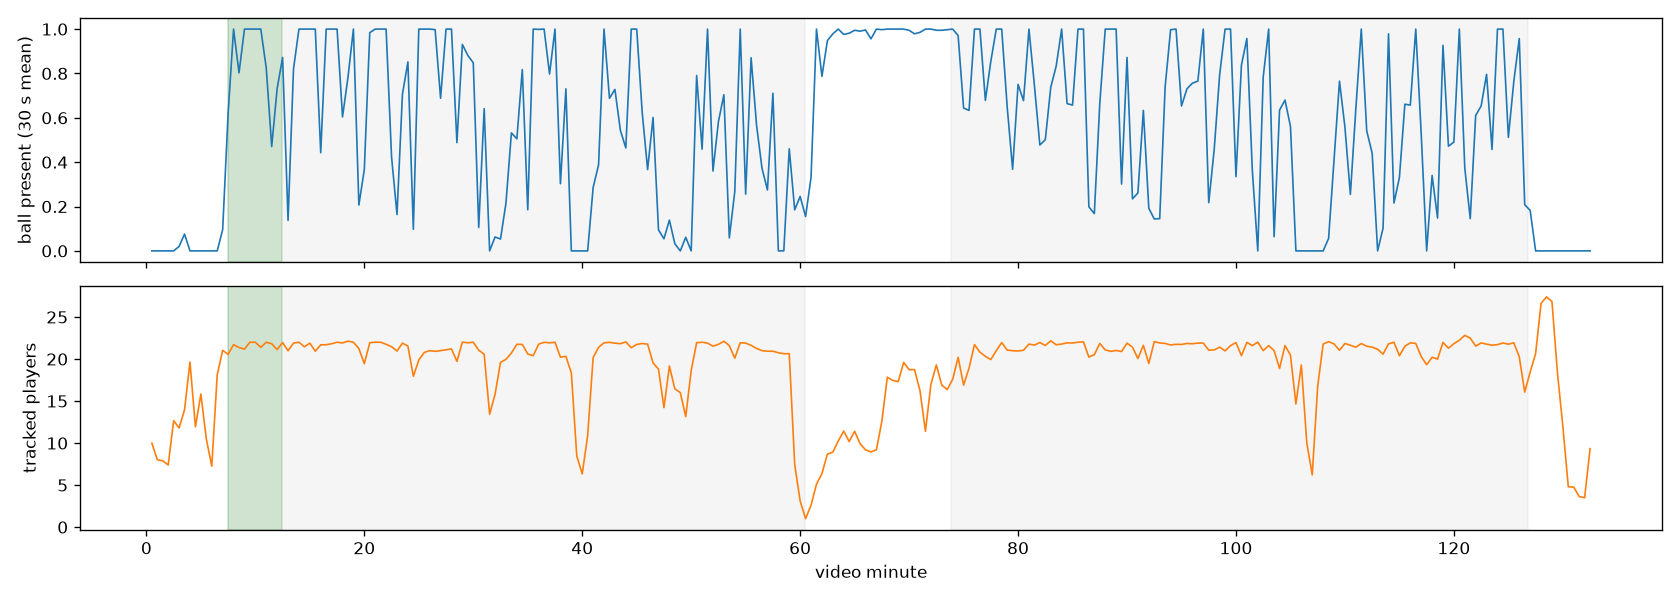
\includegraphics[width=0.92\linewidth]{ball_presence.png}
\caption{Share of frames with a tracked ball (30 s mean, top) and tracked players (bottom) over the whole video. The green band is the public window, the grey bands are the graded halves.}
\label{fig:ball}
\end{figure}

\section*{Approach}
The answer is to learn from labelled football elsewhere, made to look like this match, and to decode for the metric. Figure~\ref{fig:pipeline} shows the full pipeline. Each stage is described in the subsections below.

\begin{figure}[H]
\centering
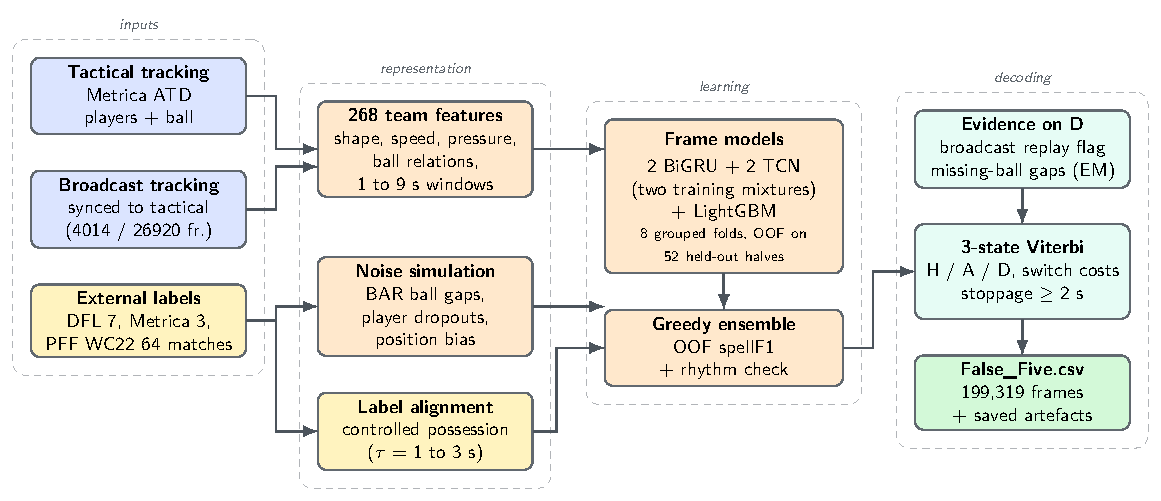
\includegraphics[width=\linewidth]{pipeline.pdf}
\caption{End-to-end pipeline. Blue boxes are the challenge inputs, yellow the external labelled data, orange the learning stages, green the decoding stages and the output.}
\label{fig:pipeline}
\end{figure}

\subsection*{Broadcast Synchronisation and the Replay Flag}
The broadcast recording turns out to be the live feed with a constant delay per half. Cross-correlating one-second means of the ball's $x$ position, then refining with a frame-level search, gives tactical frame $t$ = broadcast frame $t + 4014$ in the first half and $t + 26920$ in the second, with a median ball distance of 0.8 m where both trackings see it. This alignment unlocks two signals. First, the broadcast ball fills 8{,}049 frames where the tactical ball is missing (homography reprojection error below 5, no isolated jump above 3 m). Second, an invalid broadcast homography means the director is showing a replay or a close-up. On the public window this happens on 76\% of dead-ball frames and only 3 to 4\% of live frames, which makes it the strongest stoppage cue in the bundle.

\subsection*{External Labelled Data and Label Alignment}
Three open sources carry exactly the two quantities the ground truth is made of, a ball status and a team in possession, on full matches.

\begin{table}[H]
\centering\small
\begin{tabularx}{\linewidth}{@{}l c l X@{}}
\toprule
source & matches & tracking & possession and dead-ball labels \\
\midrule
IDSSE / Sportec DFL~[7] & 7 & optical, 25 fps, 22 players & per-frame \texttt{BallPossession} and \texttt{BallStatus} \\
Metrica sample games & 3 & Metrica tracking, 25 fps & Metrica event definitions (PASS, CARRY, RECOVERY, BALL OUT, SET PIECE, fouls) \\
PFF FC World Cup 2022 & 64 & broadcast, 29.97 fps $\to$ 25 & PFF possession sequences, \texttt{OUT} events, set-piece restarts \\
\bottomrule
\end{tabularx}
\end{table}

Raw provider labels flip on every touch (DFL changes possession 8.3 times per live minute). The challenge counts \emph{controlled} possession, so every source is aligned with one rule. A team spell shorter than $\tau$ frames is returned to the previous team when that team regains the ball or play stops right after it,
\begin{equation}
\ell_{s:e} \leftarrow \ell_{s-1} \quad \text{if} \quad e - s < \tau \;\; \text{and} \;\; \big(\ell_{e} = \ell_{s-1} \;\text{or}\; \ell_{e} = D\big),
\end{equation}
applied three times. With $\tau = 50$ frames (2 s) for DFL and Metrica and $\tau = 25$ (1 s) for PFF, all three sources reach the rhythm of the public ground truth, about 4.2 possessions per live minute with a median of 7.6 s (Figure~\ref{fig:align}). The public truth is only a reference line here. No parameter is fitted to it.

\begin{figure}[H]
\centering
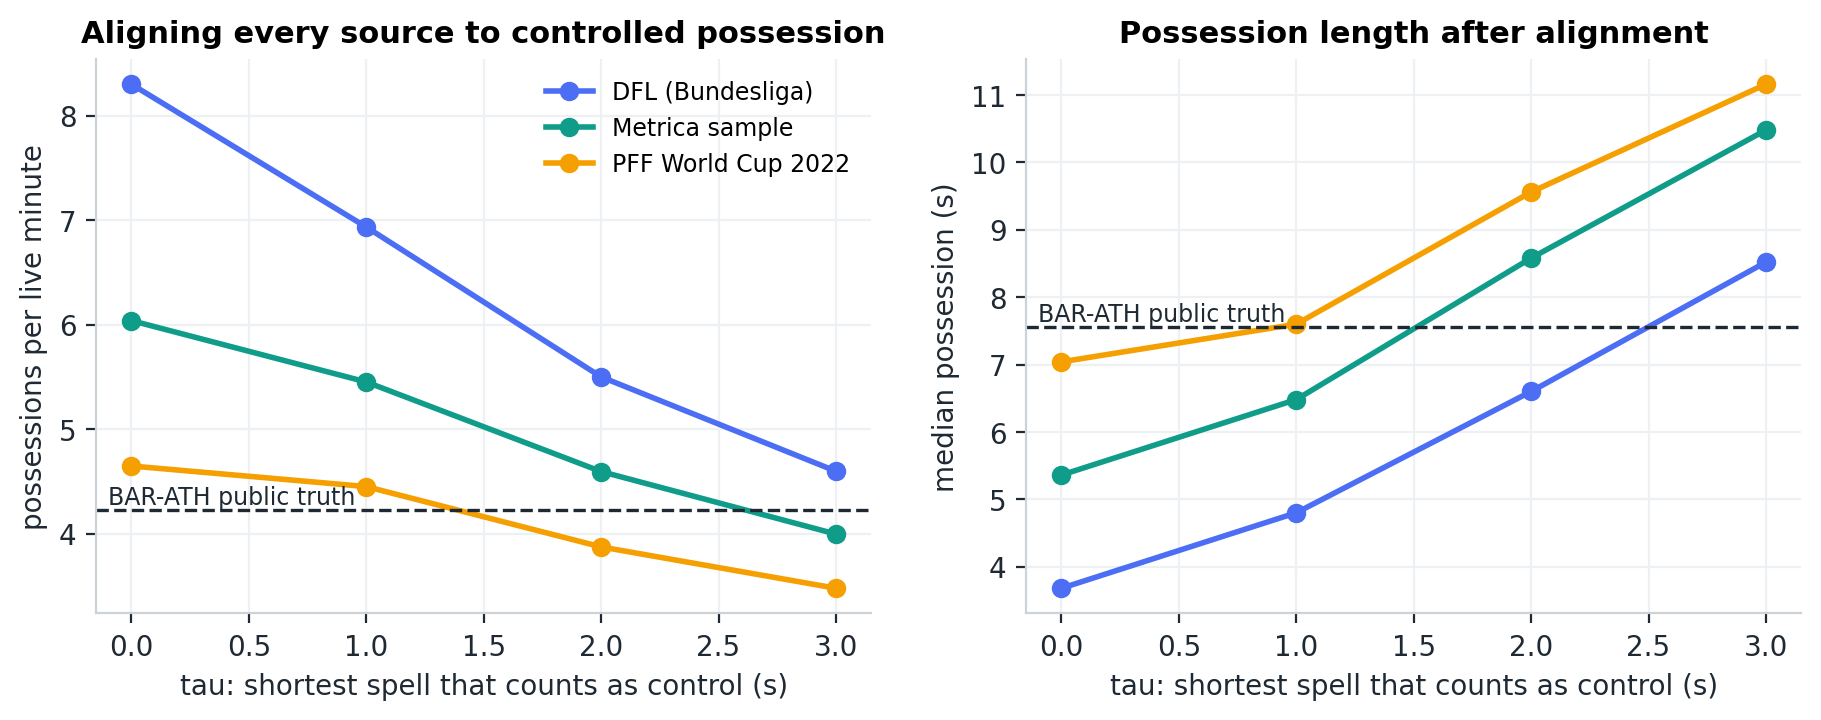
\includegraphics[width=0.9\linewidth]{label_alignment.png}
\caption{Possession rate and median length per source as a function of $\tau$, the shortest spell that counts as control. The dashed line is the BAR-ATH public ground truth.}
\label{fig:align}
\end{figure}

Each source receives a fixed share of the training weight so that PFF's 64 matches do not crowd out the others. Mixture A (DFL 35\%, Metrica 20\%, PFF 45\%) is the best all-round mix. Mixture B (DFL 45\%, Metrica 40\%, PFF 15\%) leans towards Metrica, the target's own tracker and labelling convention.

\subsection*{Simulating the Target's Noise}
The external tracking is cleaner than Metrica's automatic tracking of BAR-ATH, so every training and validation half is degraded with the target's \emph{own} noise (Figure~\ref{fig:noise}). The exact BAR-ATH ball-missing mask is copied from a random offset, so gap lengths and clustering are real. Players are dropped to match BAR-ATH's per-frame count per team in 10 s blocks. Each player receives a slowly varying position bias ($\sigma = 0.3$ m, interpolated every 2 s), which keeps speeds realistic where per-frame jitter would add fake speed. The ball gets 0.4 m of noise.

\begin{figure}[H]
\centering
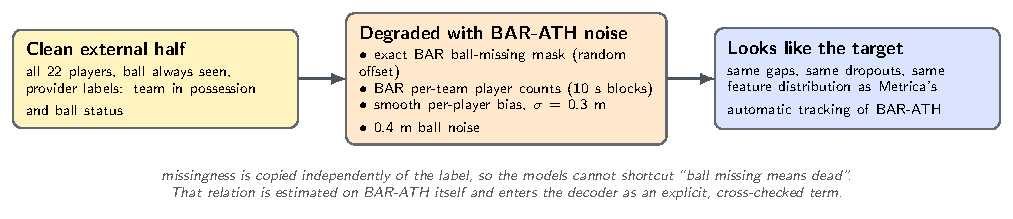
\includegraphics[width=\linewidth]{domain_transfer.pdf}
\caption{Every external half is degraded with BAR-ATH's own noise before features are computed.}
\label{fig:noise}
\end{figure}

The missing-ball mask is copied independently of the label, so the models cannot learn the shortcut ``missing ball means dead ball'', whose strength is specific to each tracker. That relation is estimated on BAR-ATH itself and enters the decoder as an explicit term.

\subsection*{Team-Level Features}
Without player identities, every one of the 268 features is team-level and permutation-invariant, in metres from the pitch centre with the home team attacking $+x$. Per team: centroid, spread, second-deepest line, most advanced player, length, width, share of players per third, mean and maximum speed, share running ($>4$ m/s) and walking ($<1$ m/s), velocity along the attacking direction, and pressure (mean distance to the nearest opponent). Speeds are also divided by the sequence's median player speed, so leagues and trackers with different absolute speeds look alike. Ball relations cover the nearest and second-nearest player per team, players within 5 m, distance outside the pitch, ball speed, and time since and until the ball was seen. All are summarised by NaN-aware rolling means over centred 1, 3 and 9 s windows and 2 and 6 s past and future windows. Swapping home and away is an exact column permutation, which doubles the training data and removes any ``home has the ball'' bias.

\subsection*{Sequence Models}
Two architectures read 5 fps sequences in 512-step chunks (102 s) and label every step. The \textbf{BiGRU} is Linear, GELU, a two-layer bidirectional GRU with hidden size 192 and a linear head, so each frame sees the whole chunk in both directions. The \textbf{TCN}~[2] stacks six residual blocks of dilated convolutions,
\begin{equation}
h^{(k+1)} = h^{(k)} + W_2\, \mathrm{GELU}\big(\mathrm{Conv}_{d_k}(\mathrm{LN}(h^{(k)}))\big), \qquad d_k \in \{1,2,4,8,16,32\},
\end{equation}
with kernel 5, giving a fixed receptive field of $1 + 4\sum_k d_k = 253$ steps, about 50 s centred on each frame. The recurrent and convolutional views of the same context make partly independent errors. Both are trained on mixtures A and B, with robust scaling, Gaussian input noise and the home/away swap. At prediction time the network runs on the five 5 fps phases of the 25 fps sequence and the outputs are interleaved. A LightGBM model~[6] on the same features (63 leaves, 300 rounds, deterministic) completes the library.

\textbf{Validation protocol.} All DFL and Metrica matches and 16 PFF matches are split into 8 grouped folds, so each is held out exactly once, and the other 48 PFF matches always train. Every model is scored out-of-fold (OOF) on identical held-out features with the official \texttt{spell\_scores} and \texttt{macro\_f1}, at two alignments per source, averaged per source, with Metrica weighted twice. The BAR-ATH prediction is the average of the eight fold models, so every probability in the submission comes from a model that was itself validated.

\subsection*{Greedy Ensemble Selection}
The ensemble is built by forward selection with replacement~[1]. Starting from nothing, each step adds one copy of the member $m$ that maximises the held-out objective after decoding,
\begin{equation}
J(w) = \text{spellF1}_{\text{OOF}}(w) - \lambda \max\!\Big(0,\; \big|\log \tfrac{r_{\text{BAR}}(w)}{r_{\text{ref}}}\big| - \log 1.1\Big),
\end{equation}
where $r_{\text{BAR}}$ is the predicted possession rate on BAR-ATH (which needs no labels), $r_{\text{ref}} = 4.45$ per live minute is the rate of the external labels and $\lambda = 0.1$. Inside the $\pm10\%$ band the penalty is zero and held-out spellF1 alone decides. The selected ensemble (Figure~\ref{fig:ens}) is BiGRU A 20\%, BiGRU B 20\%, TCN A 30\% and TCN B 30\%, with a BAR-ATH rate of 4.24, inside the band.

\begin{figure}[H]
\centering
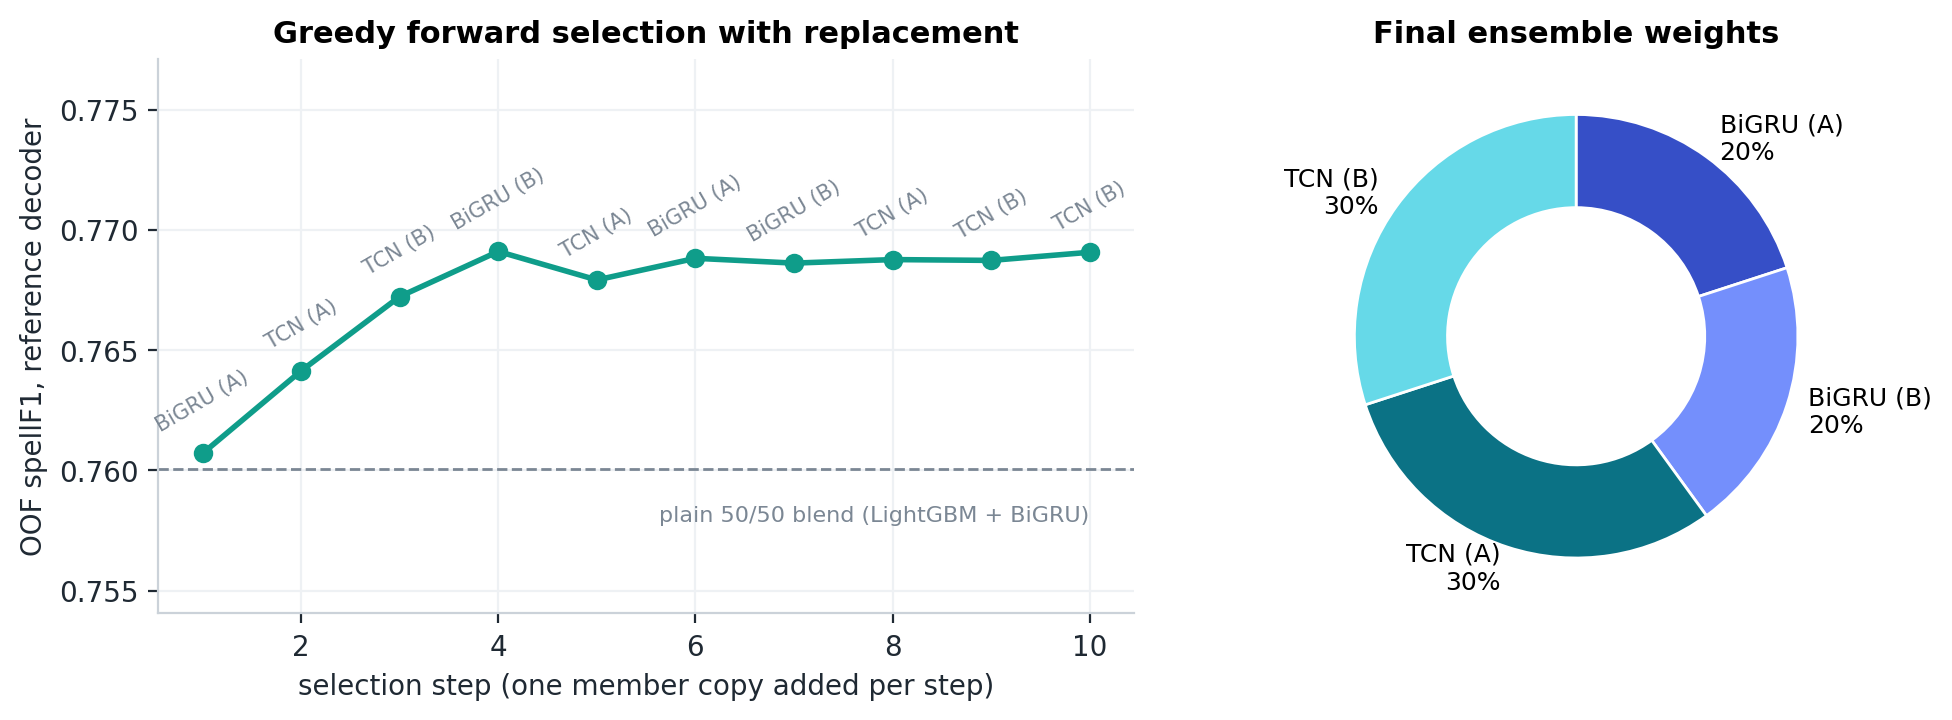
\includegraphics[width=0.9\linewidth]{ensemble.png}
\caption{Held-out spellF1 along the greedy selection path (left) and the final weights (right).}
\label{fig:ens}
\end{figure}

\subsection*{Duration-Constrained Viterbi Decoding}
Following the CRF and Viterbi view of possession~[4], the decoder finds the label sequence that maximises the per-frame log-probabilities plus evidence, minus a cost for every switch,
\begin{equation}
\hat y = \arg\max_{y_{1:T}} \sum_{t} \big[\log p(y_t \mid x) + e_t(y_t)\big] - \sum_t c(y_{t-1}, y_t) \quad \text{s.t. every } D \text{ run lasts} \geq 50 \text{ frames},
\end{equation}
with $c(H,A) = c_{\text{team}} = 12$ and $c(\cdot, D) = c(D, \cdot) = c_{\text{dead}} = 6$. The minimum stoppage of 2 s is enforced exactly by expanding $D$ into a chain of 50 sub-states (Figure~\ref{fig:dec}). The costs are chosen on held-out spellF1 over a $7 \times 5$ grid, whose surface is smooth near the optimum (Figure~\ref{fig:grid}). Each half is decoded separately, and frames outside the graded halves are \texttt{X}.

\begin{figure}[H]
\centering
\begin{minipage}{0.42\linewidth}\centering
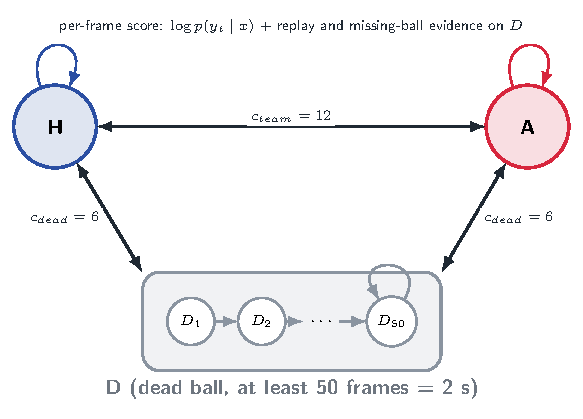
\includegraphics[width=\linewidth]{decoder.pdf}
\caption{Decoder states and switch costs.}
\label{fig:dec}
\end{minipage}\hfill
\begin{minipage}{0.55\linewidth}\centering
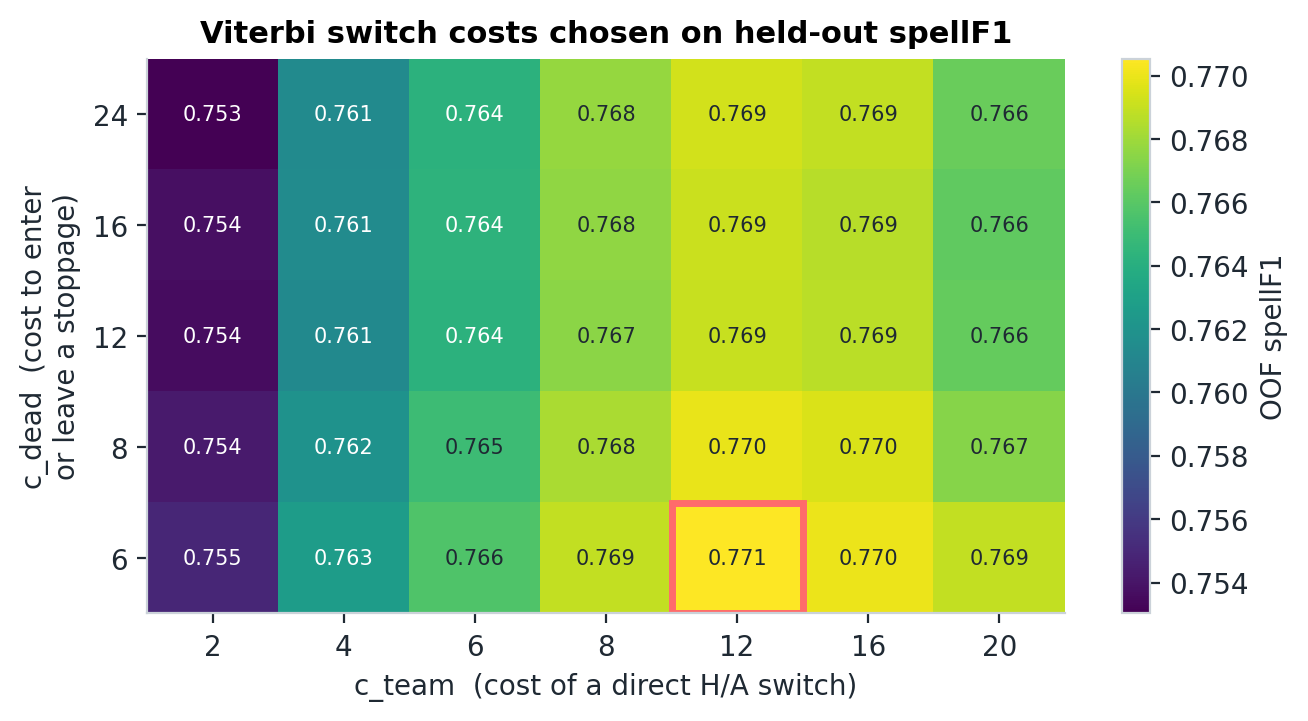
\includegraphics[width=\linewidth]{decoder_grid.png}
\caption{Held-out spellF1 over the cost grid. The red box is the chosen setting.}
\label{fig:grid}
\end{minipage}
\end{figure}

\subsection*{Match-Specific Evidence on the Dead-Ball State}
Two signals exist only for this match. Both enter as $e_t(D)$.

\textbf{Replay.} Under a naive-Bayes view, the broadcast flag $f_t$ adds $\log P(f_t \mid D) - \log P(f_t \mid \text{alive})$. The public-window log-ratios are $+3.1$ (replay) and $-1.4$ (live picture). Half of each, $+1.5$ and $-0.7$, is used so as not to over-trust four stoppages.

\textbf{Missing-ball gaps.} Each graded frame gets a category $g_t$: ball visible, or the length of the gap it lies in (under 0.5 s, 0.5 to 2 s, 2 to 5 s, 5 to 10 s, 10 to 30 s, over 30 s). With dead-ball posteriors $q_t$ from the model-only decode, one EM step gives
\begin{equation}
e^{\text{gap}}(g) = \tfrac{1}{2}\left[\log \frac{\sum_t q_t\, [g_t = g]}{\sum_t q_t} - \log \frac{\sum_t (1-q_t)\, [g_t = g]}{\sum_t (1 - q_t)}\right].
\end{equation}
A visible ball argues for live play ($-0.99$ before shrinkage) and gaps over 30 s strongly for a stoppage ($+4.33$, Figure~\ref{fig:gap}), matching video spot checks of drinks breaks, substitutions and goal celebrations. The term is kept only if it improves agreement with the replay flag, which is not used in its estimate. It does, raising the replay log-likelihood from $-0.465$ to $-0.459$. Each signal referees the other, and neither is tuned on the public window.

\begin{figure}[H]
\centering
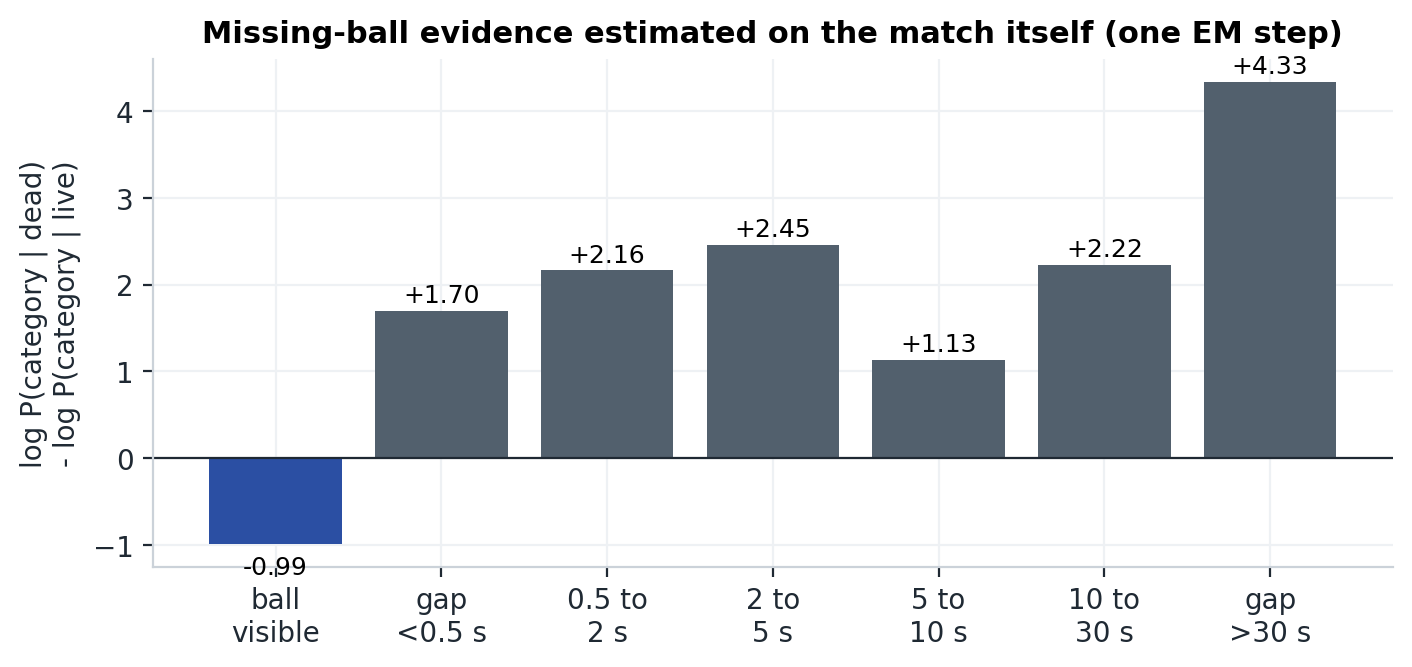
\includegraphics[width=0.6\linewidth]{gap_evidence.png}
\caption{Missing-ball log-ratios estimated on BAR-ATH by one EM step.}
\label{fig:gap}
\end{figure}

\section*{Possession Rules}
The rules follow from the label sources (DFL \texttt{BallStatus}, Metrica's event definitions, PFF \texttt{OUT} events and set-piece types), aligned to one notion of control in the spirit of Link and Hoernig~[5], and reinforced by the decoder (Figure~\ref{fig:rules}).

\begin{figure}[H]
\centering
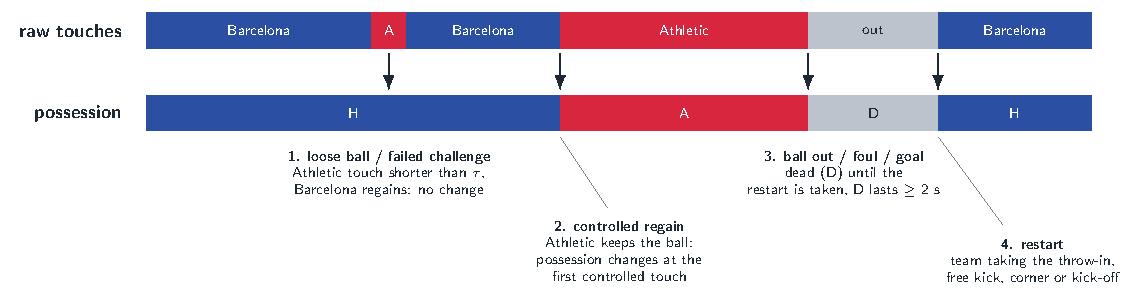
\includegraphics[width=\linewidth]{possession_rules.pdf}
\caption{From raw touches to possession: loose balls and failed challenges, a controlled regain, a stoppage and a restart.}
\label{fig:rules}
\end{figure}

\begin{itemize}[leftmargin=1.2em]
\item \textbf{Controlled possession.} A team has the ball from its first controlled action until the opponent gains control or play stops. A spell shorter than $\tau$ (2 s, or 1 s for PFF sequences) that ends with the previous team regaining the ball is a touch, not a possession.
\item \textbf{Loose balls.} Deflections, blocked passes and balls in the air stay with the last team in control until the opponent establishes control. The switch cost $c_{\text{team}}$ adds the same inertia at prediction time.
\item \textbf{Challenges.} A tackle changes possession only when the winning team keeps the ball. A duel won and immediately lost does not flip possession.
\item \textbf{Stoppages.} The ball is dead from the moment it leaves the pitch, or from the referee's stoppage for a foul, offside, goal or injury, until the restart is taken. A stoppage lasts at least 2 s.
\item \textbf{Restarts.} Throw-ins, corners, goal kicks, free kicks, penalties and kick-offs give possession to the team taking them from the moment the ball is back in play.
\end{itemize}

\section*{Validation and Results}
\begin{table}[H]
\centering\small
\begin{tabular}{@{}lccccc@{}}
\toprule
model & DFL & Metrica & PFF & weighted spellF1 & macroF1 \\
\midrule
LightGBM & 0.709 & 0.761 & 0.633 & 0.716 & 0.901 \\
BiGRU, mixture A & 0.750 & 0.799 & 0.696 & 0.761 & 0.918 \\
BiGRU, mixture B & 0.719 & 0.789 & 0.657 & 0.738 & 0.914 \\
TCN, mixture A & 0.707 & 0.755 & 0.687 & 0.726 & 0.915 \\
TCN, mixture B & 0.705 & 0.766 & 0.669 & 0.727 & 0.912 \\
\midrule
\textbf{Ensemble + decoder + evidence} & \textbf{0.750} & \textbf{0.814} & \textbf{0.705} & \textbf{0.771} & \textbf{0.923} \\
\bottomrule
\end{tabular}
\caption{Out-of-fold spellF1 on 52 held-out halves (14 DFL, 6 Metrica, 32 PFF), each degraded with BAR-ATH's noise. Frame accuracy of the final system is 92.2\%.}
\end{table}

\textbf{Public window (official scorer).} spellF1 \textbf{0.688} (bootstrap 5 to 95\%: 0.51 to 0.86), 62\% above the best baseline (0.424), and 0.81 at IoU 0.3. macroF1 \textbf{0.927} (H 0.948, A 0.925, D 0.907), frame accuracy 93.3\%, Cohen's $\kappa$ 0.892, alive/dead F1 0.979. All four stoppages are found, 15 possessions are predicted against 17, and the median boundary latency is +2 frames (Figure~\ref{fig:pub}).

\begin{figure}[H]
\centering
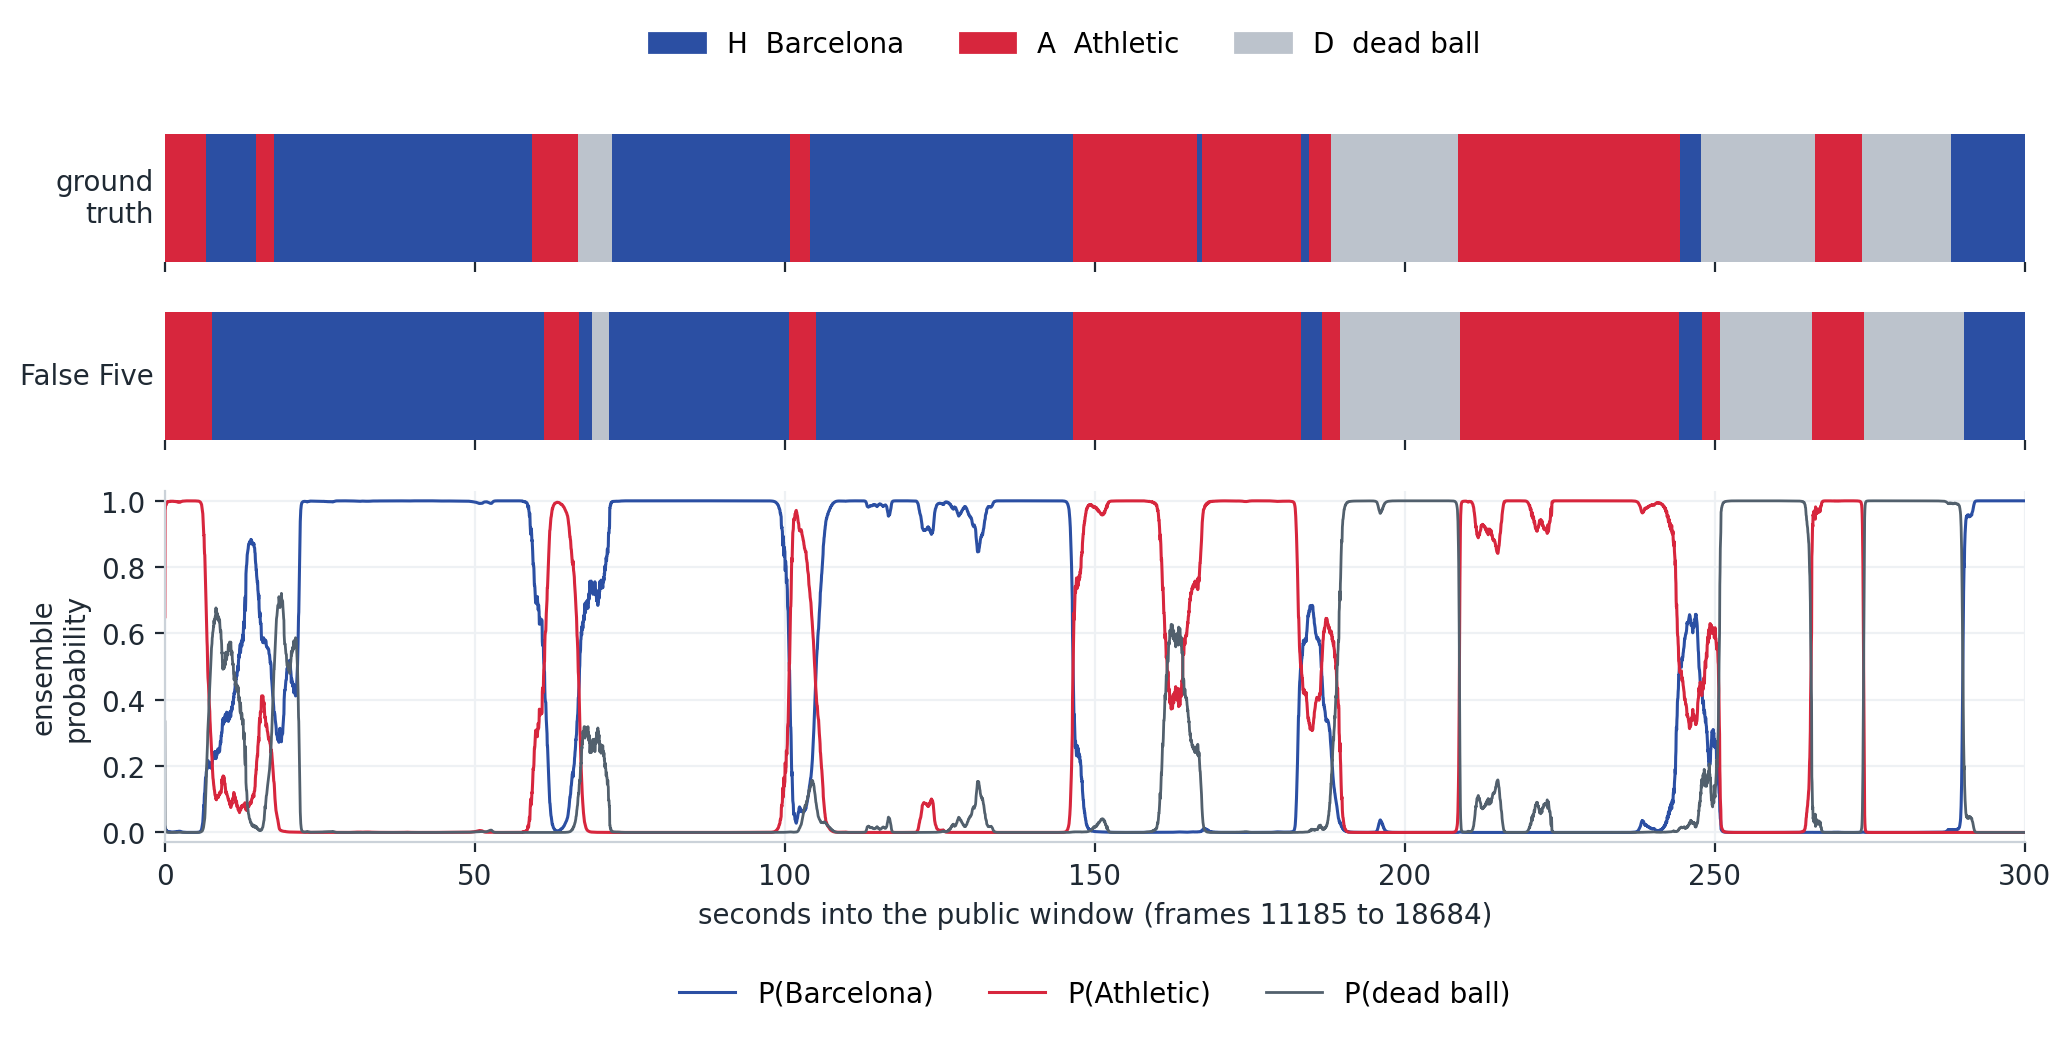
\includegraphics[width=\linewidth]{public_window.png}
\caption{Public window. Ground truth (top), our submission (middle) and the ensemble probabilities (bottom).}
\label{fig:pub}
\end{figure}

\textbf{Full match.} 216 possessions, 3.98 per live minute (public truth 4.23), mean length 15.1 s (public truth 14.2 s), 109 stoppages and a dead-ball share of 48.8\%, close to LaLiga's typical effective playing time of about 50\%. Barcelona holds 63.4\% of live ball. On held-out halves, the median boundary offset is within 2 frames for team changes, stoppages and restarts on all three sources (Figure~\ref{fig:timing}), so no systematic shift is needed.

\begin{figure}[H]
\centering
\begin{minipage}{0.56\linewidth}\centering
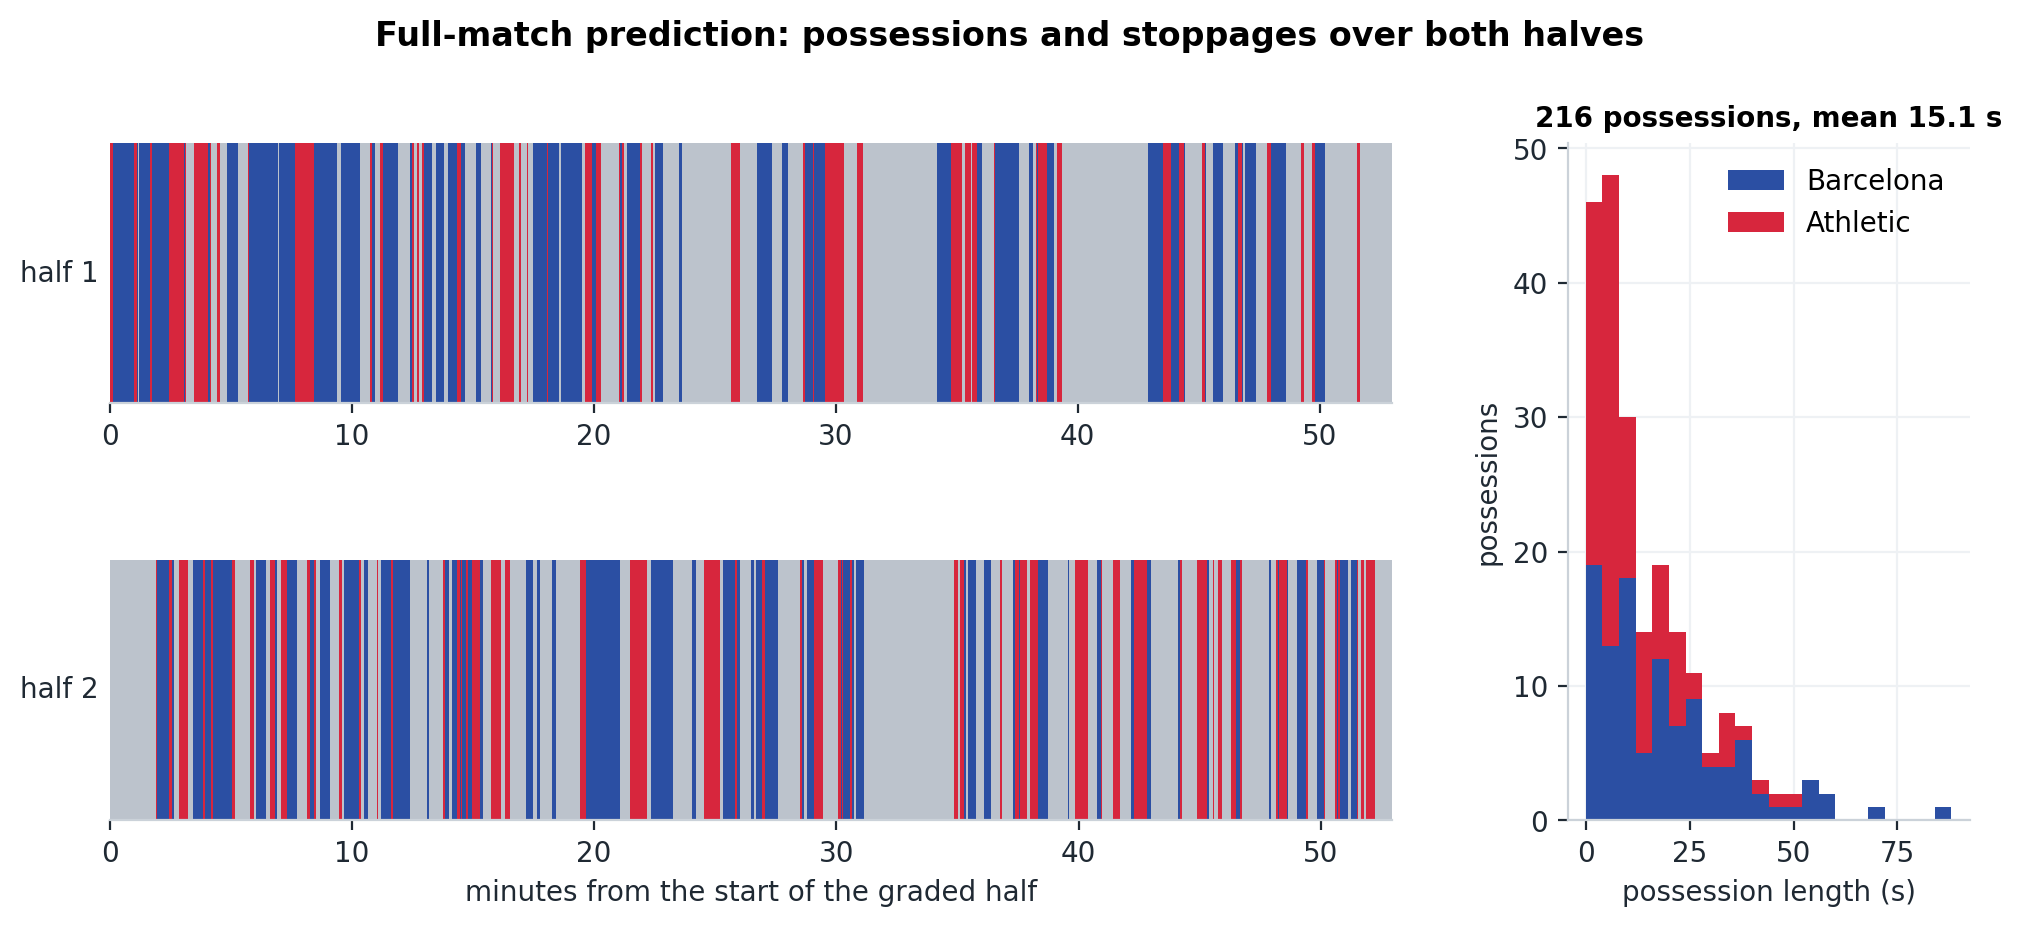
\includegraphics[width=\linewidth]{full_match.png}
\end{minipage}\hfill
\begin{minipage}{0.42\linewidth}\centering
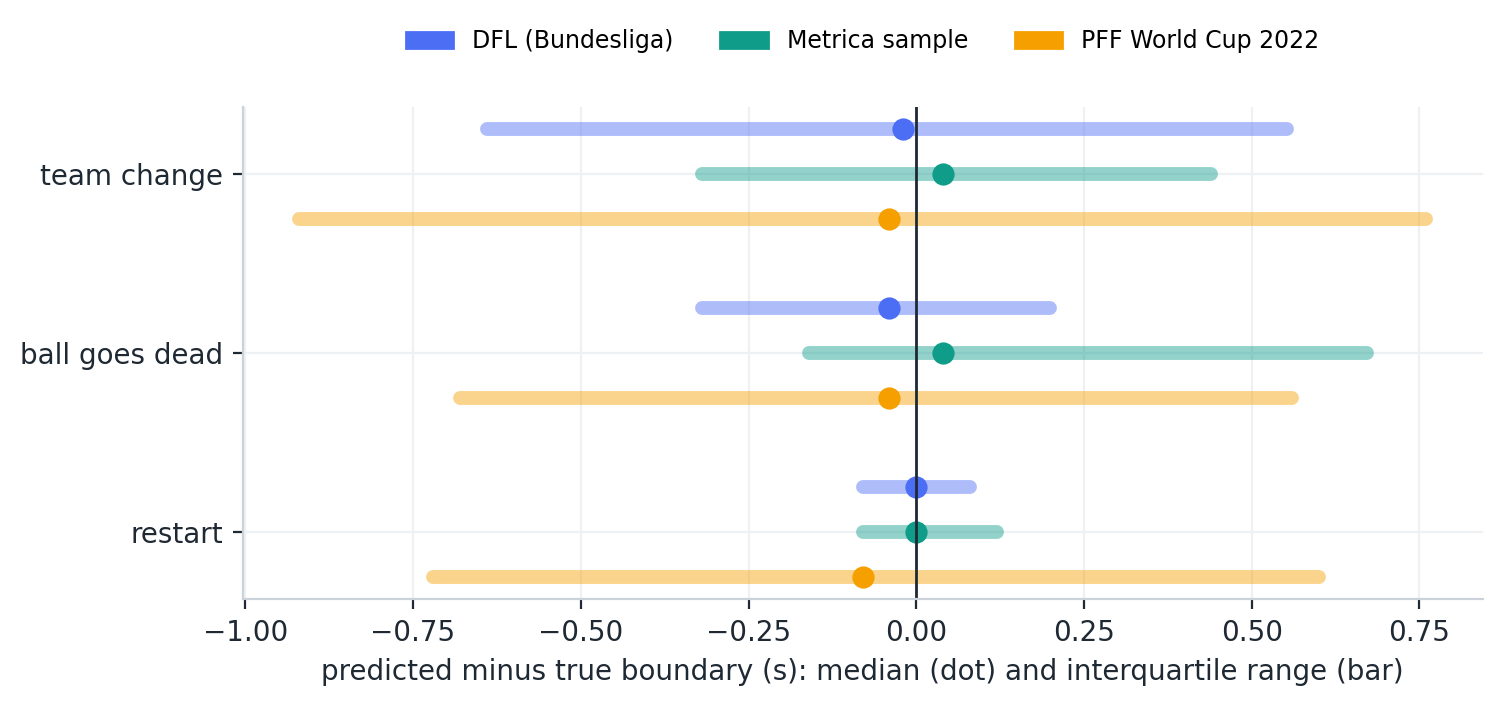
\includegraphics[width=\linewidth]{boundary_timing.png}
\end{minipage}
\caption{Full-match prediction with the possession length histogram (left) and held-out boundary timing per transition type and source (right).}
\label{fig:timing}
\end{figure}

\section*{Assets Used}
\begin{table}[H]
\centering\small
\begin{tabularx}{\linewidth}{@{}l X@{}}
\toprule
asset & how it is used \\
\midrule
Tactical ATD and metadata & all 268 features, slot teams, attack direction \\
Broadcast ATD and homography & 8{,}049 gap-filled ball frames and the replay flag \\
Public 5-minute ground truth & reporting and the replay log-ratios only, never for model or decoder selection \\
Official scorer and validator & every metric in this document and the final format check \\
IDSSE / Sportec DFL open data & training and validation (CC-BY 4.0) \\
Metrica Sports sample data & training and validation, the closest proxy for the target \\
PFF FC World Cup 2022 & training (64 matches) and validation (16), free after registration with PFF FC \\
\midrule
Smart Tagging & left out: its fixed-length windows agree with the public truth on about 70\% of live frames \\
Tactical video pixels & left out: the tracking summarises the video and the replay flag captures stoppages cheaply \\
\bottomrule
\end{tabularx}
\end{table}
No private ground truth, hand labelling or manual correction is used. Every submitted label comes out of the algorithm in the repository.

\section*{Limitations and Future Potential}
The external labels come from events (Metrica, PFF) or from another provider's tracking (DFL), none from Metrica's corrected tracking that defines the ground truth, so the notion of control is learned through alignment rather than directly. A handful of labelled matches in the target convention would sharpen it. The largest remaining uncertainty sits in long live-play ball gaps, where a football ball detector on the 1080p tactical frames could recover the ball. Player-level set transformers feeding the temporal models, trained end to end with a CRF over \texttt{H}/\texttt{A}/\texttt{D}~[3,4], and a label-conditional gap simulation calibrated on BAR-ATH are natural next steps. Each one plugs into the same held-out protocol, which tells immediately whether it helps.

\section*{Reproduction}
The last pipeline step is deterministic, so the notebook saves its inputs (ensemble probabilities, evidence on $D$ and decoder settings). The submission is rebuilt byte for byte on any CPU in about 10 seconds:
\begin{shellcode}
pip install -r requirements-regenerate.txt
python regenerate_submission.py
# sha256 427dc39b0fafc4c950ce4de7fd210dd26219429d964ba5aa631743badb2d3581
# byte-identical to False_Five.csv: True
\end{shellcode}
The full pipeline runs from raw data with \texttt{notebooks/false\_five\_possession.ipynb} (one RTX 5090, about 4 to 5 hours, Python 3.12, PyTorch 2.11, LightGBM 4.6):
\begin{shellcode}
pip install -r requirements.txt
export MTAH_DATA_DIR=/path/to/data  MTAH_REF_DIR=/path/to/reference
export MTAH_REPO_DIR=/path/to/more-than-a-hack-2027
jupyter nbconvert --to notebook --execute notebooks/false_five_possession.ipynb
\end{shellcode}
Seeds are fixed, LightGBM is deterministic and PyTorch runs in deterministic mode. The notebook re-runs the regeneration script and asserts that its output is identical to the submission.

\section*{References}
\begin{itemize}[leftmargin=2em]
\item[{[1]}] R. Caruana, A. Niculescu-Mizil, G. Crew, and A. Ksikes, ``Ensemble selection from libraries of models,'' in \textit{Proc. ICML}, 2004.
\item[{[2]}] S. Bai, J. Z. Kolter, and V. Koltun, ``An empirical evaluation of generic convolutional and recurrent networks for sequence modeling,'' arXiv:1803.01271, 2018.
\item[{[3]}] M. Borghesi \textit{et al.}, temporal convolutional networks for team possession and ball status estimation, \textit{Expert Systems with Applications} 223, 119780, 2023.
\item[{[4]}] H. Kim \textit{et al.}, PathCRF, ball-free possession inference with a CRF and Viterbi decoding, arXiv:2602.12080, KDD 2026.
\item[{[5]}] D. Link and M. Hoernig, ``Individual ball possession in soccer,'' \textit{PLoS ONE} 12(7), 2017.
\item[{[6]}] G. Ke \textit{et al.}, ``LightGBM: a highly efficient gradient boosting decision tree,'' in \textit{Proc. NeurIPS}, 2017.
\item[{[7]}] M. Bassek, R. Rein, H. Weber, and D. Memmert, ``An integrated dataset of spatiotemporal and event data in elite soccer,'' \textit{Scientific Data}, 2025.
\end{itemize}

\end{document}
